%\documentclass[journal,twocolumn,10pt]{IEEEtran}
\documentclass[conference]{IEEEtran}
\usepackage{amsmath}
\usepackage{hhline}
%\usepackage{graphicx}
\usepackage[dvips]{graphicx} %  !!!!!!!!!!!!!!!!!!!
%for png files, use \includegrpahics[nathwith=<XX>bp, natheight=<YY>bp, width=<width>]{filename.png}
\usepackage{bmpsize} % for png compiling !!!!!!!!!!!!!
\usepackage{epsfig}
\usepackage{multirow}
\usepackage{setspace}
\usepackage{color}
\usepackage{url}
\usepackage{caption}
\usepackage{subcaption}
\usepackage{enumerate}
\usepackage{amsfonts}
\usepackage{amsthm}
\usepackage{amscd}
\usepackage{amssymb}
\usepackage[left=0.75in, right=0.75in, top=1in, bottom=0.75in]{geometry}

\begin{document}
	
	%%%%%%%%% TITLE
	\title{Causal Models}
	
	\author{\IEEEauthorblockN{Kenneth Lai\textsuperscript{1,2} and Svetlana Yanushkevich\textsuperscript{1}}
		\IEEEauthorblockA{\textsuperscript{1}Biometric Technologies Laboratory, Department of Electrical and Software Engineering, University of Calgary, Canada\\ 
			\IEEEauthorblockA{\textsuperscript{2}Department of Clinical Neurosciences, Cumming School of Medicine, University of Calgary, Canada\\ 
				Email: \{kelai, syanshk\}@ucalgary.ca}}
	}	
	
	\markboth{IEEE}{ \MakeLowercase{\textit{et al.}}:
		.....}
	
	\maketitle
	
	\begin{abstract}
		The impacts of mass migration, such as crises induced by climate change, extend beyond environmental concerns and can greatly affect social infrastructure and public services, such as education, healthcare, and security. These crises exacerbate certain elements like cultural barriers and discrimination by amplifying the challenges faced by these affected communities. This paper proposes an innovative approach to address migration crises in the context of crisis management through a combination of modeling and imbalance assessment tools. By employing deep learning for forecasting and integrating causal reasoning via Bayesian networks, this methodology enables the evaluation of imbalances and risks in the socio-technological landscape, providing crucial insights for informed decision-making. Through this framework, critical systems can be analyzed to understand how fluctuations in migration levels may impact them, facilitating effective crisis governance strategies.
				
	\end{abstract}
	
	\begin{IEEEkeywords}
		Migration, Forecasting, Deep Learning, Machine Reasoning, Bayesian Networks.
	\end{IEEEkeywords}
	
	\section{Introduction}
	
	\begin{figure}[!htb]
		\begin{center}
			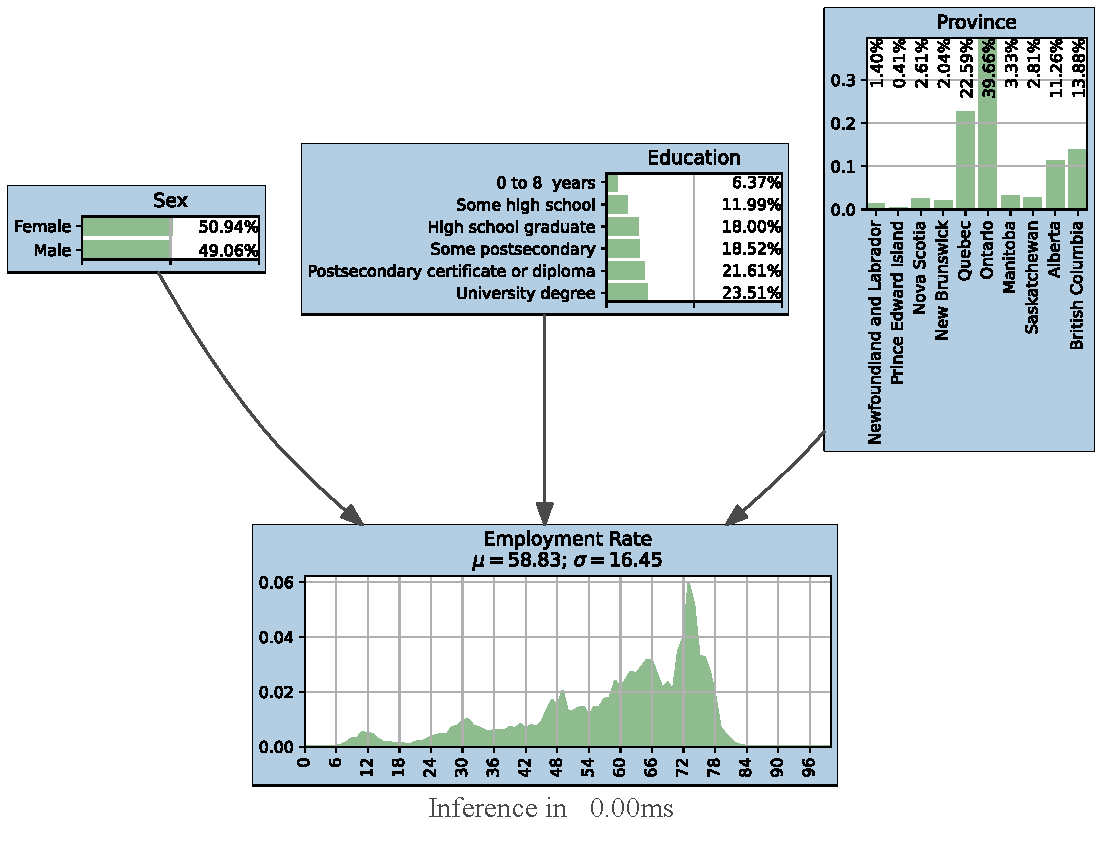
\includegraphics[clip, trim= 0 0 0 0, width=0.49\textwidth]{fig/bn_edu.pdf}
			\caption{}
			\label{fig:1}
		\end{center}
	\end{figure}
	
	\begin{figure}[!htb]
		\begin{center}
			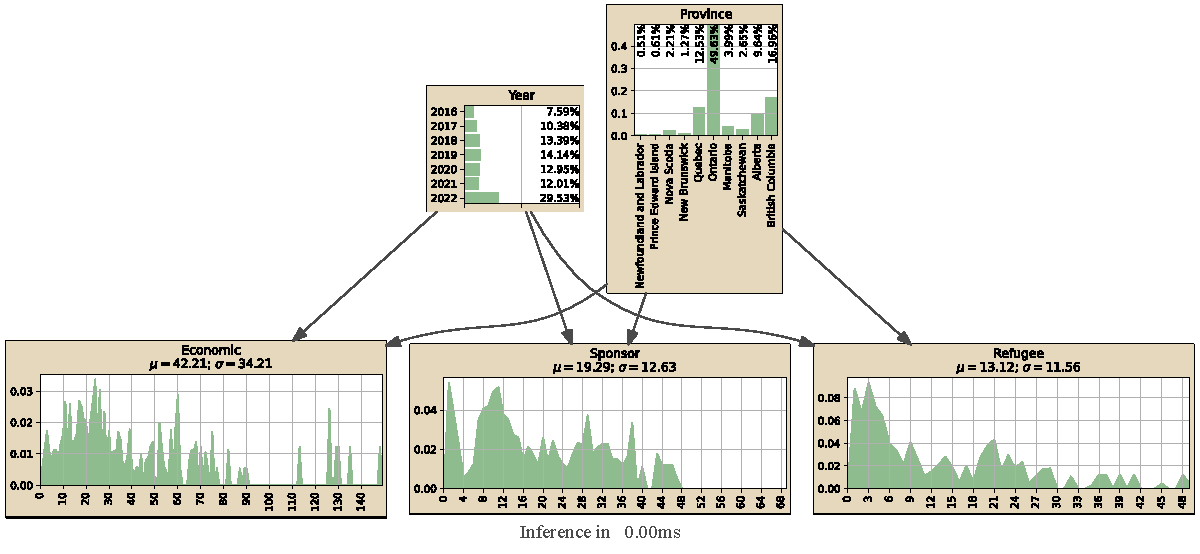
\includegraphics[clip, trim= 0 0 0 0, width=0.49\textwidth]{fig/bn_pr.pdf}
			\caption{}
			\label{fig:2}
		\end{center}
	\end{figure}
	
	\begin{figure}[!htb]
		\begin{center}
			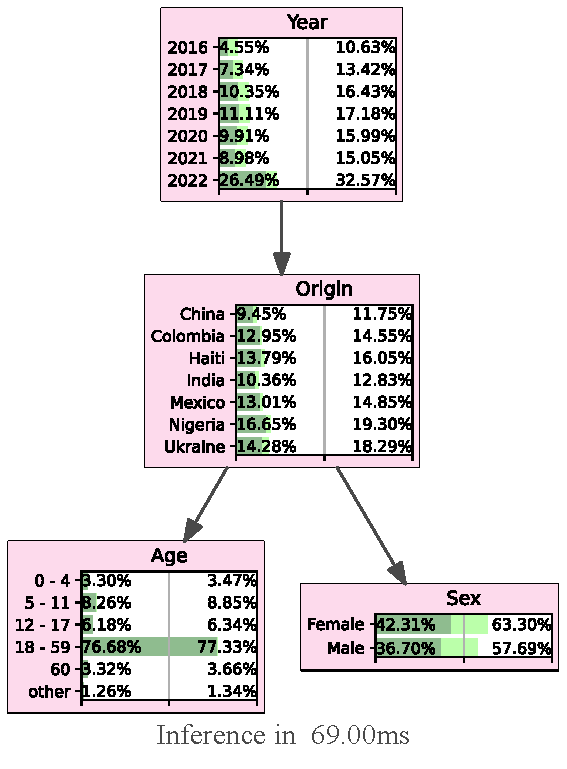
\includegraphics[clip, trim= 0 0 0 0, width=0.49\textwidth]{fig/credal_refugee.pdf}
			\caption{}
			\label{fig:3}
		\end{center}
	\end{figure}
	
	\begin{figure}[!htb]
		\begin{center}
			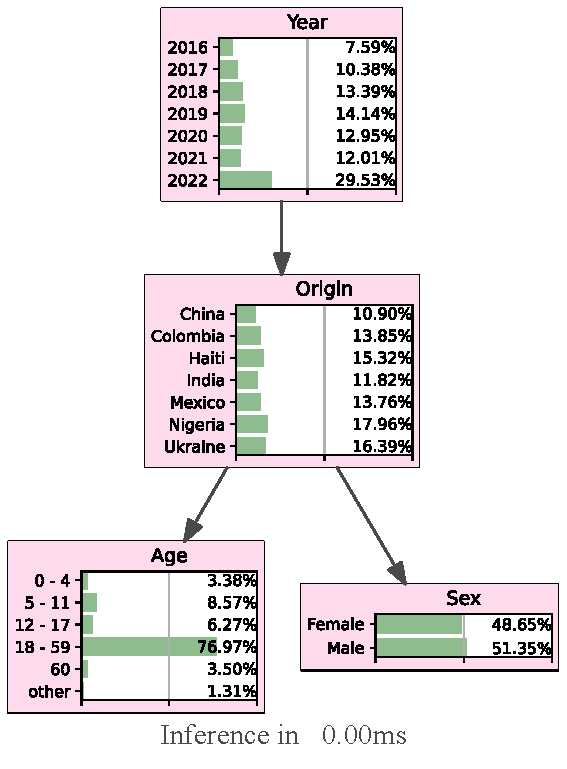
\includegraphics[clip, trim= 0 0 0 0, width=0.49\textwidth]{fig/bn_refugee.pdf}
			\caption{}
			\label{fig:4}
		\end{center}
	\end{figure}
	
	\begin{figure*}[!htb]
		\begin{center}
			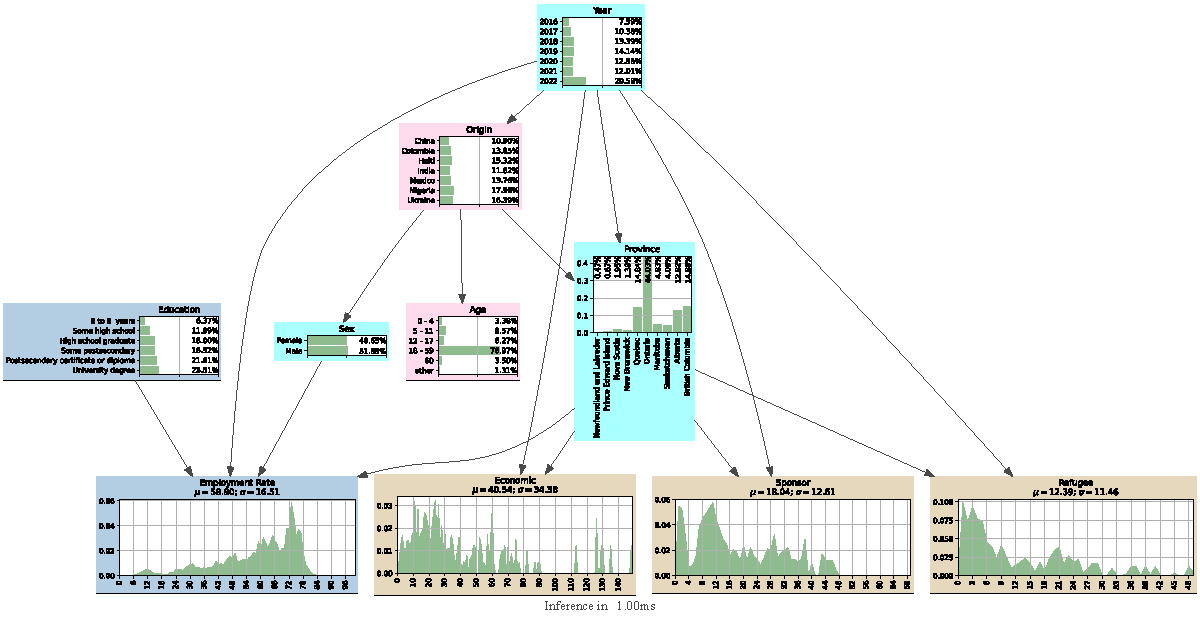
\includegraphics[clip, trim= 0 0 0 0, width=0.99\textwidth]{fig/bn_refugee+pr+edu.pdf}
			\caption{}
			\label{fig:5}
		\end{center}
	\end{figure*}
	
	
	\section{Discussion and Conclusion}
	
	
	\subsection*{Acknowledgment}
	
	\begin{small}
		This work was supported in part by the Social Sciences and Humanities Research Council of Canada (SSHRC) through the Grant ``Emergency Management Cycle-Centric R\&D: From National Prototyping to Global Implementation'' under Grant NFRF-2021-00277; in part by the University of Calgary under the Eyes High Postdoctoral Match-Funding Program.
	\end{small}
	
	
	{\small
		\bibliographystyle{IEEEtran}
		\bibliography{bib}
	}
	
\end{document}